\documentclass[conference]{IEEEtran}

\usepackage[utf8]{inputenc}
\usepackage{cite}
\usepackage{graphicx}
\graphicspath{{figs/}}
\DeclareGraphicsExtensions{.pdf,.jpg,.png}

\usepackage[caption=false,font=footnotesize]{subfig}
\usepackage{url}
\hyphenation{op-tical net-works semi-conduc-tor}


\begin{document}
%
% paper title
% can use linebreaks \\ within to get better formatting as desired
\title{Natural Interaction for Object Hand-Over}


\author{\IEEEauthorblockN{Mamoun Gharbi, Séverin Lemaignan, Jim Mainprice, Rachid Alami}
\IEEEauthorblockA{CNRS-LAAS, 7 av. du Colonel Roche, F-31077 Toulouse, France\\
Université de Toulouse, UPS, INSA, INP, ISAE, LAAS, F-31077 Toulouse, France\\
Email: {\tt surname.name@laas.fr}}
}
% make the title area
\maketitle


\begin{abstract}

The video presents in a didactic way several abilities and algorithms
required to achieve interactive ``pick and give'' tasks in a human environment.
Communication between the human and the robot relies on unconstrained verbal
dialogue, the robot uses multi-modal perception to track the human and its
environment, and implements real-time 3D motion planning algorithms to achieve
collision-free and human-aware interactive manipulation.

\end{abstract}


%This film covers recent results from the LAAS-CNRS laboratory in the field of
%\emph{interactive manipulation with companion robots}. 
We tackle here the issue of \emph{natural} and \emph{legible} behaviour for a
robot intended to live in domestic environment, amongst human peers.
\emph{Natural} because we aim at unconstrained spoken English mixed with
gestures and perspective taking to communicate with the robot ; \emph{legible}
because we apply human-aware motion planning algorithms that ensure a smooth
human-robot interaction by accounting for implicit social rules which appear in
placement or approach strategies.

\vspace{1em}

%The video demonstration is the result of the integration of many different
%components: we focus here on modules dedicated to high-level motion planning
%and decision making 

\begin{figure}[h!]
        \centering
        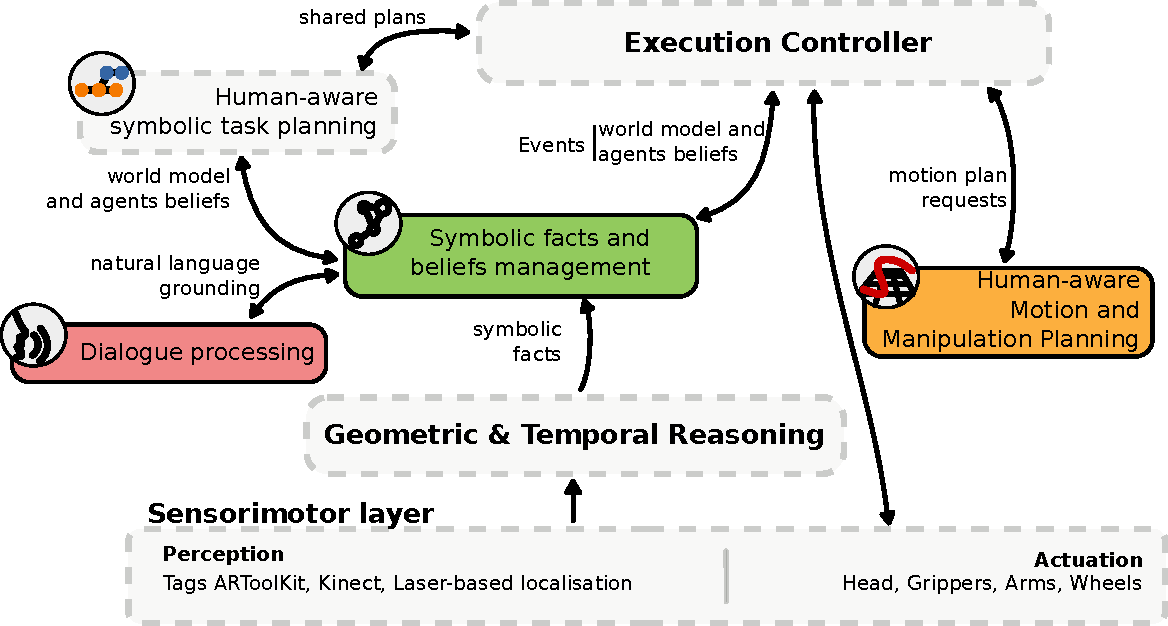
\includegraphics[width=0.9\columnwidth]{archi}
        \caption{Overview of the robot deliberative
        architecture~\cite{Alami2011a}. Coloured modules with plain borders are
        the specific focus of the video.}
        \label{fig|archi}
\end{figure}

\subsection{Modelling of the environment}

The video clip gives a overview of the techniques used on-line by the robot
to build a model of its environment. We rely first on a geometric model, fed by
Kinect-like sensors for human tracking and 2D barcodes for object identification
and localization.

From this geometric model, we build in real-time a symbolic model, stored as an
ontology~\cite{Lemaignan2010}. This models holds spatial relations between
objects and agents, along with a set of \emph{affordances} (like reachability,
visibility, etc.) \cite{Lemaignan2011a}.

\subsection{Natural language processing}

The video also introduces recent work on natural dialogue
grounding~\cite{Lemaignan2011a}. The user verbal input is first parsed, then
semantically grounded, in tight interaction with the symbolic model. It allows
for multi-modal and perspective-aware communication: affordances (like
visibility) and human gestures that are recognized (like pointing) and stored
in the ontology are used during the grounding process.

\subsection{Motion planning in human close vicinity}

While planning the robot motions, it is important to account for interaction constraints  such as those defined by the proxemics theory. Motion planning techniques such as the ones in \cite{Mainprice:11}  enable to
account for such constraints using a cost-based representation where efficient algorithms incorporating features from stochastic
optimization are applied to produce low-cost paths. 

\subsection{Sharing effort in handover tasks and proactive robot placement}

The planner demonstrated in this video has been introduced in \cite{Mainprice:12}, it also accounts for interaction constraints. It consists of sampling handover configurations encoding for the human and robot postures ensuring that they are accessible to them both. The configurations are evaluated regarding an interaction cost and the one that minimizes this cost is returned by the planner. This algorithm enables the robot to proactively decide where to give the object. It can produce plans either for a seated or standing human or through a window as shown in the video. 
We have introduced a notion of \textit{mobility} to tune the amount of effort asked to the human. 
%\subsection{Human-aware trajectory planning for hand-over}

\section*{Acknowledgment}

This work has been supported by EU FP7 ``SAPHARI'' under grant agreement no. ICT-287513.

\bibliographystyle{IEEEtran}
\bibliography{IEEEabrv,biblio,bib_jim}

% that's all folks
\end{document}


